\documentclass[12pt]{article}

\usepackage[margin=1in]{geometry}
\usepackage{setspace}
\usepackage{amsmath}
\usepackage{fancyhdr}
\usepackage{xcolor}
\usepackage{graphicx}
\usepackage{float}
\usepackage{sidecap}


\setlength{\headheight}{15.2pt}
\pagestyle{fancy}


\newcommand{\quotes}[1]{``#1''}

\lhead{}
\chead{}
\rhead{Zeno's Paradox of the Dichotomy \ \ \ \thepage}
\lfoot{}
\cfoot{}
\rfoot{}
\renewcommand{\headrulewidth}{0pt}

\begin{document}

\begin{center}
	\textcolor{white}{a} \\
	\vspace{15\baselineskip}
	\Large {Zeno's Paradox of the Dichotomy: A Mathematical Analysis} \\
	\vspace{.8cm}
	\Large {Andrew Wang} \\
	\vspace{.8cm}
	\Large{Mr. Waithe} \\
	\vspace{.8cm}
	\Large{MPM 2D7} \\
\end{center}


\newpage

\doublespacing
\indent Infinity is an abstract idea that describes something with unbounded value. It is involved in many famous paradoxes, thought experiments and has it has its applications in modern day calculus and physics. Throughout history, it has been a controversial topic. The ancient Greeks, the Pythagoreans, outlawed the infinite and the irrational in their mathematical society. Since childhood, infinity has truly fascinated me. It is one of the things that I can wonder about all afternoon without ever seeming to get bored of it, albeit my knowledge of infinity has not always been very clear. Although, its mysticism is indubitably appreciable. Recently, I encountered the famous Zeno's paradox of the dichotomy, one of Zeno of Elea's paradoxes of motion. It features Achilles, Greek hero of the Trojan War. Simply put, Achilles attempts to finish a footrace in pieces. He starts by completing half the race. Every subsequent section is half the distance of the previous section. Zeno asserts that since there are an infinite number of sections to the race, it cannot be finished (Alper, J.S., \& Bridger, 1997, p. 144). This paradox baffles (and slightly frustrates) me| when I first discovered it I could explain neither its obvious flawed logic nor its apparent correctness. In this mathematical exploration, I aim to examine and comment on this paradox that combines mathematics, science, and philosophy alike. 


\indent Suppose that Achilles has to run a 100 metre long footrace. Say, also, that he runs in sections. He starts by travelling one half of the race, halts, then continues for a quarter, then an eighth, and so on. The paradox is that since the distance Achilles has left to travel can always be further divided in two, he will never reach the finish line. This conclusion is quite peculiar because it is apparent that we can finish races in real life. For example, sprinters who participate in the Olympics have been known to complete footraces in rather short periods of time. So why then, does the logic of the paradox seem to be correct?

\begin{figure}[H]
  \begin{minipage}[c]{0.67\textwidth}
    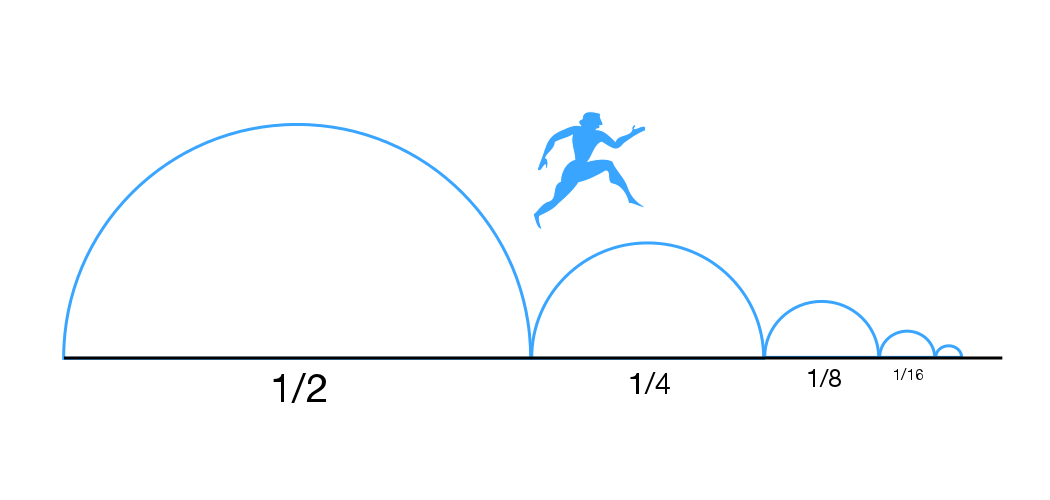
\includegraphics[width=\textwidth]{Zeno_Dichotomy_Paradox.png}
  \end{minipage}\hfill
  \begin{minipage}[c]{0.3\textwidth}
    \caption{
 A diagram showing the pieces of the race that Achilles must complete.
    } 
  \end{minipage}
\end{figure}

\indent Mathematically, we can represent the distance that Achilles travels as a geometric series. That is to say that it is the sum of a sequence of infinite numbers generated with a starting number and a common ratio. This model reflects the fact that in the paradox, it is stated that Achilles has infinite segments to travel. Each subsequent term is yielded by multiplying the preceding term by the common ratio. Consider the following examples of geometric series: 
\begin{eqnarray}
3 + 6 + 12 + 24 + 48 + 96 \\
1 + 1 + 1 + 1 + 1 + 1 \\
9 + 3 + 1 + \frac{1}{3} +  \frac{1}{9} + \frac{1}{27}
\end{eqnarray}

	Notice that dividing some term $u_n$, where n is the term number of sequence $u$ and n $>$ 0, by $u_{(n-1)}$ equals a constant ratio, r. In (1), the starting term (a) is 3 and the ratio (r) is 2; in (2), a = 1, r = 1; in (3), a = 9, r= 1/3. In general, an infinite geometric series can be represented as: 
					$$S=a+ar+ar^2+〖ar〗^3\ldots$$
	where $a$ is the start term and $r$ is the common ratio. 
		In the case of Zeno's Paradox of the Dichotomy, the common ratio is one half, since each section of the race is one half the distance of the previous section. Each subsequent distance is generated by multiplying the previous distance by 0.5. The first section of the race is one half of 100 metres long, which is 50 metres. The geometric series that models Zeno's paradox is as follows: 
\begin{eqnarray*}
S&=&50 + 25 + 12.5 + 6.25 + 3.125\ldots \\
&=&50 + 50\left(\frac{1}{2}\right) + 50\left(\frac{1}{2}\right)^2 + 50\left(\frac{1}{2}\right)^3 + 50\left(\frac{1}{2}\right)^4 \ldots
\end{eqnarray*}

		These calculations were not performed in vain, though, because now we can take the partial sums of the series and see what values we get. The partial sum of sequence, as the name suggests, is the sum of a portion of the sequence only. For example, summing the first three terms of the series, 50, 25, and 12.5, equals 87.5. Summing the first four terms of the series, 50, 25, 12.5, 6.25, equals 93.75. Notice that as more terms are included into the partial sum, the sum's value increases, logically. However, since each term's magnitude diminishes (the common ratio has magnitude less than 1), the series will converge. That is to say that with more and more terms, the series approaches closer and closer to a definite value because each successive term impacts the overall sum less and less. This can be shown by manipulating the general form of a geometric progression to yield the partial sum formula. A geometric progression differs from a geometric series in that it sums a sequence of a finite number of terms, as opposed to a sequence of an infinite number of terms.
\begin{equation*}
	\begin{split}
			S ={}& a + ar + ar^2 + ar^3 \ldots + ar^{n-1} \\
			rS ={} & ar + ar^2 + ar^3 \ldots + ar^{n-1}+ ar^n \\
			S - rS ={} & a + ar + ar^2 +{ar}^3 \ldots ar^{n-1} \\
			& \; \! - (ar + ar^2 +{ar}^3 \ldots ar^{n-1} + ar^n)
	\end{split}
\end{equation*}
		Subtracting like terms vertically, we end up with every cancelled except for a and $ar^n$. Notice that for a geometric sequence of n terms, the last term is $ar^{n-1}$ and not $ar^n$. This is because the first term is $ar^0$, as opposed to $ar^1$.
\begin{eqnarray*}
	S(1-r)&=& a-ar^n \\
	&=& a (1-r^n) \\ 
	S &=& a \left(\frac{1-r^n}{1-r}\right), r \neq 1 \\
\end{eqnarray*}
\indent	For $|r| < 1$ and $n \geq 0$, the value of the rational expression does not \quotes{explode}. This is also seen when taking the limit of the expression as n approaches infinity. The limit of a function is the value that its output approaches as its input approaches some number(Stewart, 2008). A limit of a function is notated as follows: 
$$\lim_{x \to c}f(x) = L$$

	This is the limit, $L$, of the function $f(x)$ as the input, $x$ approaches $c$, assuming $L$ exists (the function is continuous in neighbouring area).

	In our case, we're looking at the expression $1-r^n$ (the numerator) for very large values of $n$. We can then take the limit of the expression as n approaches infinity.
\begin{eqnarray*}
	\lim_{n \to \infty}(1-r^n) =&=& 1-0 \\
	 &=& 1
\end{eqnarray*}
		Given that $|r|<1$, greater and greater values of n only decrease the magnitude of $r^n$. Say that $r$ is represented as a ratio between $a$ and $b$ where $b > a > 1$. When $r$ is raised to the $n^{th}$ power where $n > 1$, $b$ outgrows $a$. The closer $n$ approaches infinity, the more $b^n$ overpowers $a^n$, and thus, the closer $r^n$ approaches 0, and the numerator, $1 - r^n$ approaches 1.  This proves that a geometric series with a common ratio of magnitude less than one will converge. 
		
		We can now apply the partial sum formula to Zeno's paradox of the dichotomy and take the limit of the expression as the number of terms, n, in the partial sum approaches infinity.
\begin{eqnarray*}
\lim_{n\to\infty} \left[50\left(\frac{1-\left(\frac{1}{2}\right)^n}{1-\frac{1}{2}}\right)\right] &=& 50\left(\frac{1-0}{\frac{1}{2}}\right) \\
&=&50(2)\\
&=&100\\
\end{eqnarray*}
		This result mathematically represents Zeno's paradox| after an infinite number of sections, Achilles can finish his race. This is seen from the limit taken of the partial sum formula. However, taking the limit of the expression only tells us that with larger and larger values of n, the partial sum approaches 100. At a finite number n, such as 1000, Achilles has not yet travelled 100 metres. Since Achilles cannot travel an infinite number of sections, he can never fully finish the race, then. This result does not hold true in the real world, though. This is because we cannot grant infinitely divisible length, which is a requirement of the paradox. Upon reflection, is it possible to move one 1000th of a centimetre? Likely not. 
		
\indent Physicists tell us that the shortest meaningful length, in the real world, is the Planck length: $10^{-33}$ centimetres (Waldrop, 1990). And so, given that it is incoherent to move less than a Planck length, Achilles will reach a point where the distance between his position and the finish line is no longer divisible. With the next section of his travel, he will cross the finish line. 

\indent In writing this mathematical exploration, I applied my knowledge of geometric series to model Achilles' movement in one of Zeno's paradoxes of motion. I learned about limits, and discussed my result and its real world implications. However, my analysis of the Paradox of the Dichotomy only begins to scratch the surface of that which can be mathematically analysed as such. For example, a supertask is a series of infinite process, or steps, that is completed within a finite period of time. A notable example of a supertask is Thomson's lamp. A lamp is turned on and off an infinite amount of time in two minutes. Thomson asks what state the lamp is in after the two minutes: on or off (Berresford, G. C.. (1981). 

\indent On a final note, a question: \quotes{why do we care about paradoxes}? What does it matter, if Achilles can or cannot finish his race? Surely, whether Thomson's lamp is on or off after two minutes is insignificant? 

\indent Thousands of years ago, the Neanderthals and homo sapiens coexisted for at least 5000 years. Although, an intriguing difference between the two species was that Neanderthals did not move very far. They explored until there was either water, or some other significant obstacle. Homo sapiens, on the other hand, did things that made no sense| they dared to question the unknown and cross terrain and water without knowing what lay ahead.  As pointed out by Svante Pabo, the head Max Planck Institute for Evolutionary Anthropology, in Leipzig, \quotes{I like to think or say, some madness there. You know? How many people must have sailed out and vanished on the Pacific before you found Easter Island? I mean, it's ridiculous. And why do you do that? Is it for the glory? For immortality? For curiosity? And now we go to Mars. We never stop.} (Kolbert, 2011) After all, it was the Neanderthals who went extinct, not the modern human. If you want to solve problems, you don't just solve the ones that are already there. You make and find more, going after the impossible. 


\newpage

\begin{thebibliography}{3}
\bibitem[1]{Alper}
	Alper, J. S., \& Bridger,
	M.. (1997). 
	Mathematics, Models and Zeno's Paradoxes. Synthese,
	110(1), 143 | 166.
	Retrieved from http://www.jstor.org/stable/20117589
	
\bibitem[2]{Berresford}
	Berresford, G. C.. (1981). 
	A Note on Thomson's Lamp 'Paradox'. Analysis, 41(1), 
	1|3. http://doi.org/		
	10.2307/3327861

\bibitem[3]{Stewart}
	Stewart, J. (2008).
	Calculus: Early transcendentals.
	Belmont,
	CA: Thomson Brooks/Cole. 
	
\bibitem[4]{Waldrop}
	Waldrop,
	M. M.. (1990). 
	Viewing the Universe as a Coat of Chain Mail.
	Science, 250(4987),
	1510 | 1511.
	Retrieved from http://www.jstor.org/stable/2878321
	
\bibitem[5]{Kolbert}
	Kolbert, E. 
	(2011, August 15). 
	Sleeping with the Enemy.
	Retrieved May 03, 2016, 
	from http://www.newyorker.com/magazine/2011/08/15/sleeping-with-the-enemy

\end{thebibliography}

\end{document}
